\documentclass[11pt]{article}
\usepackage{amsmath}
\usepackage{graphicx}
\usepackage{geometry}
\geometry{a4paper, margin=0.5in}

\title{Solutions to HW\#4 \\ \large Homework for Chapter 9}
\author{JC Vaught}
\date{Due by 2:50 pm on Tuesday, Nov 12, 2024}

\begin{document}

\maketitle
\subsection*{Question 1a: Phases and Composition at Point C (5 points)}
A copper-nickel alloy phase diagram is shown below.
\newline\textbf{What are the phases and what is the composition of each phase at Point C?}

\begin{itemize}
    \item \textbf{Phases Present:} $\alpha + L$ (Solid + Liquid)
    \item \textbf{Composition of Phases at Point C:}
    \begin{itemize}
        \item \textbf{Liquid Phase:} 27 wt\% Ni
        \item \textbf{$\alpha$ Phase:} 38 wt\% Ni
    \end{itemize}
\end{itemize}

\noindent\textit{Description of Derivation:} To determine the phases and their compositions at Point C, we draw a horizontal line at Point C until it intersects the liquidus and solidus lines. From these intersection points, we then draw vertical lines down to the composition axis. The intersection with the liquidus line gives approximately 27 wt\% Ni, and the intersection with the solidus line gives approximately 38 wt\% Ni.

\begin{figure}[h!]
    \centering
    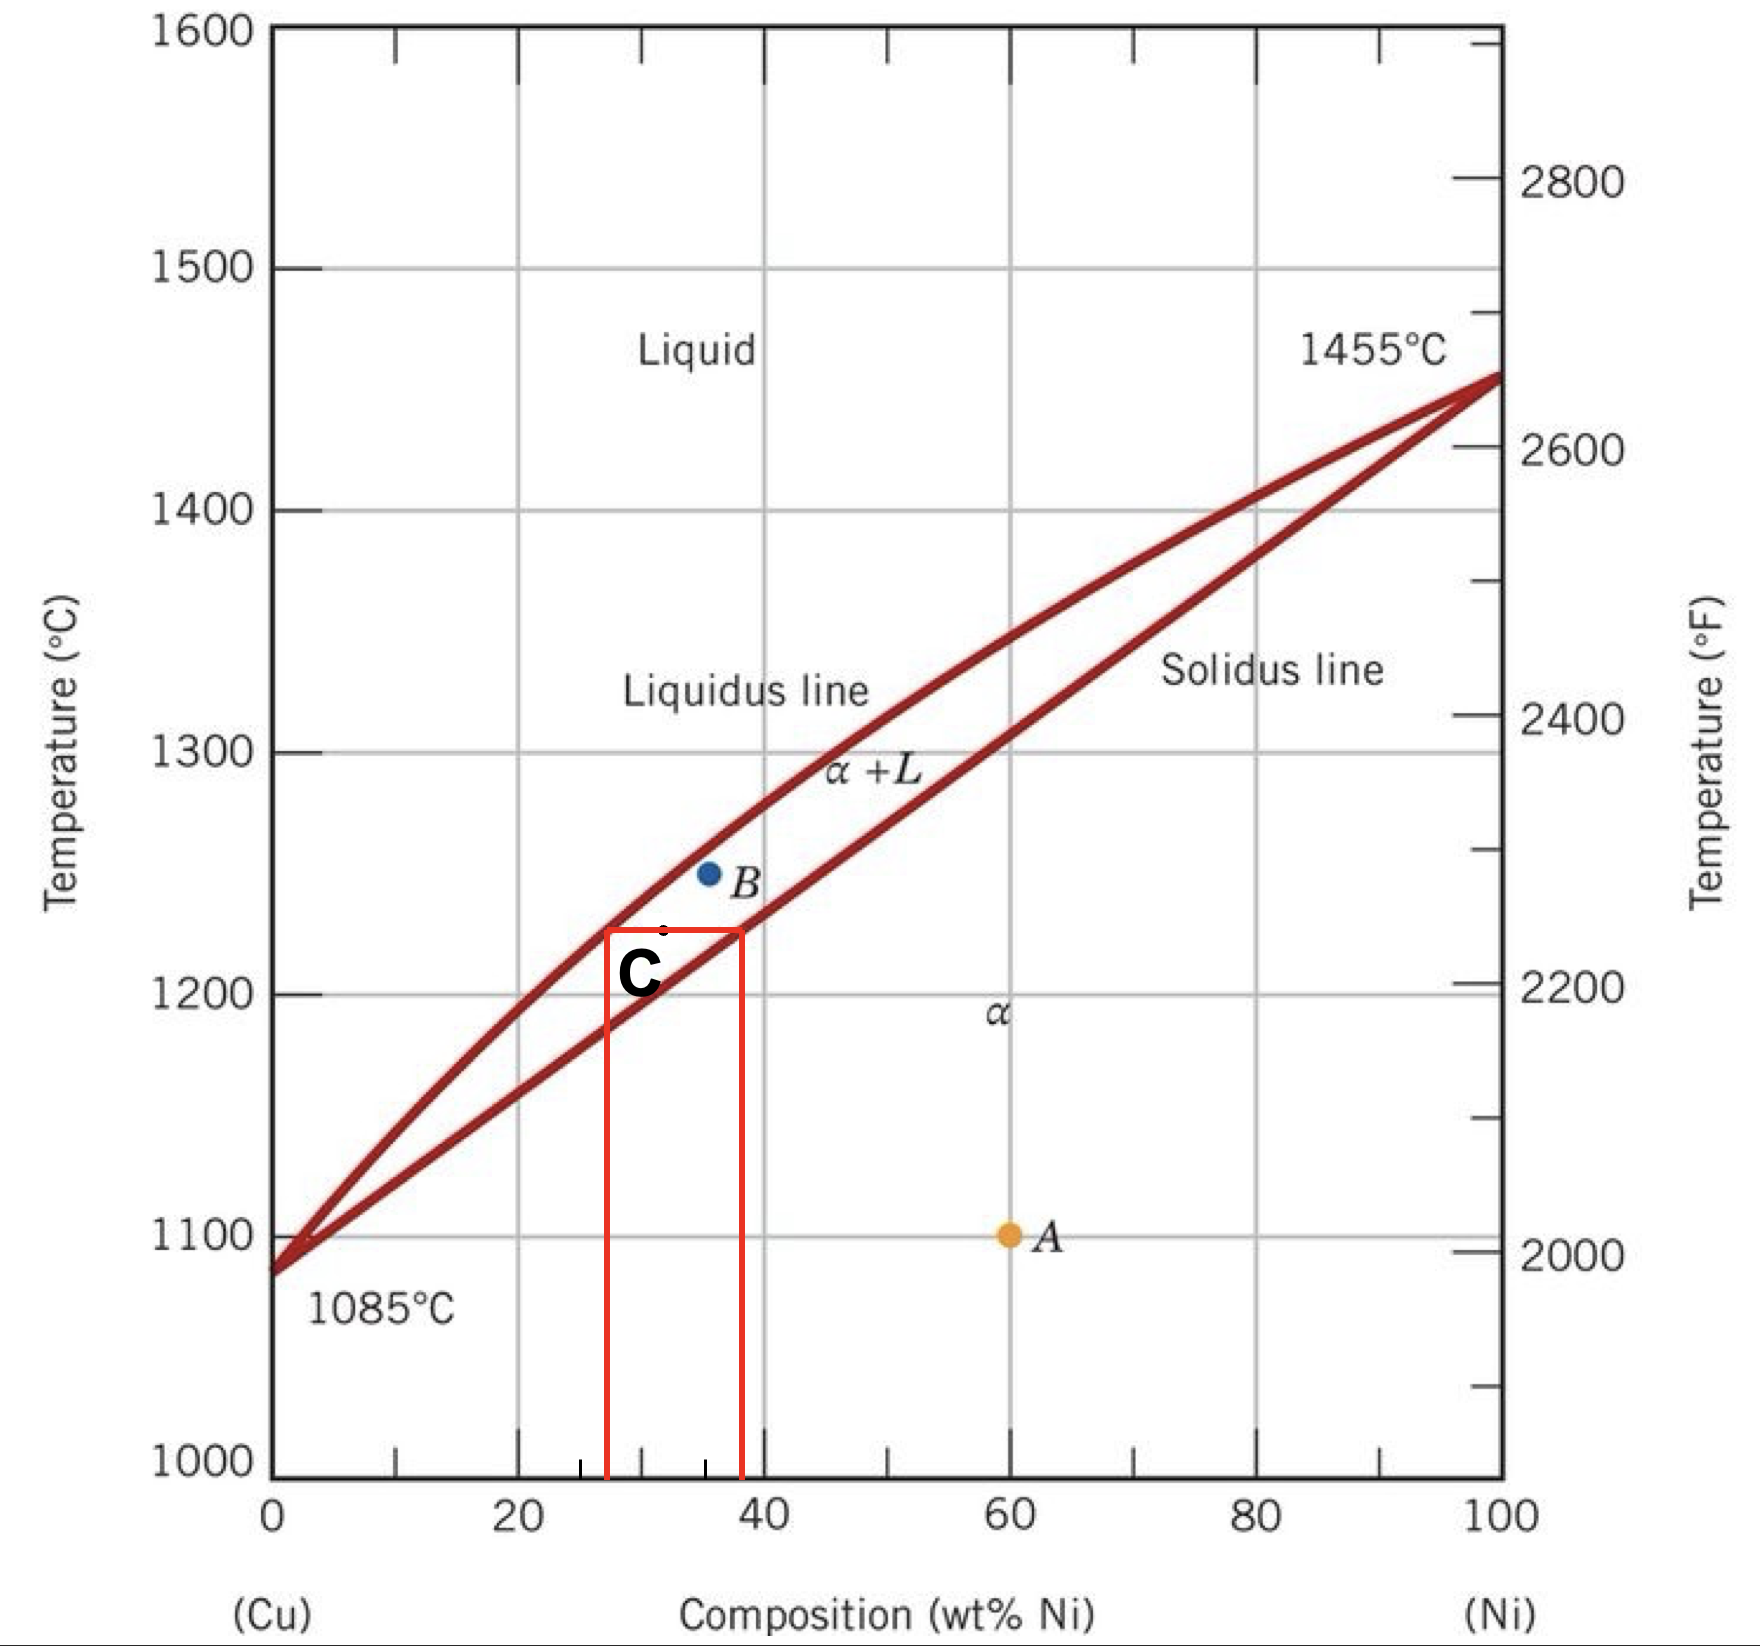
\includegraphics[width=0.7\textwidth]{hw4i1.png}
    \caption{Copper-Nickel Alloy Phase Diagram at Point C}
\end{figure}

\subsection*{Question 1b: First Liquid Phase Formation (5 points)}
A copper-nickel alloy with a composition of 80 wt\% Ni is slowly heated from room temperature to 1500~$^\circ$C.
\textbf{At what temperature does the first liquid phase form, and what is its composition?}

\begin{itemize}
    \item \textbf{Temperature of First Liquid Phase Formation:} $\sim$1380~$^\circ$C
    \item \textbf{Composition of First Liquid Phase:} $\sim$71 wt\% Ni
\end{itemize}

\noindent\textit{Description of Derivation:} Drawing a vertical line at 80 wt\% Ni until it intersects the solidus line, we then draw a horizontal line to determine the temperature axis, which is approximately 1380~$^\circ$C. We also look where this vertical line intersects the liquidus line and draw another vertical line to the composition axis, determining that the composition of the first liquid phase is approximately 71 wt\% Ni.

\begin{figure}[h!]
    \centering
    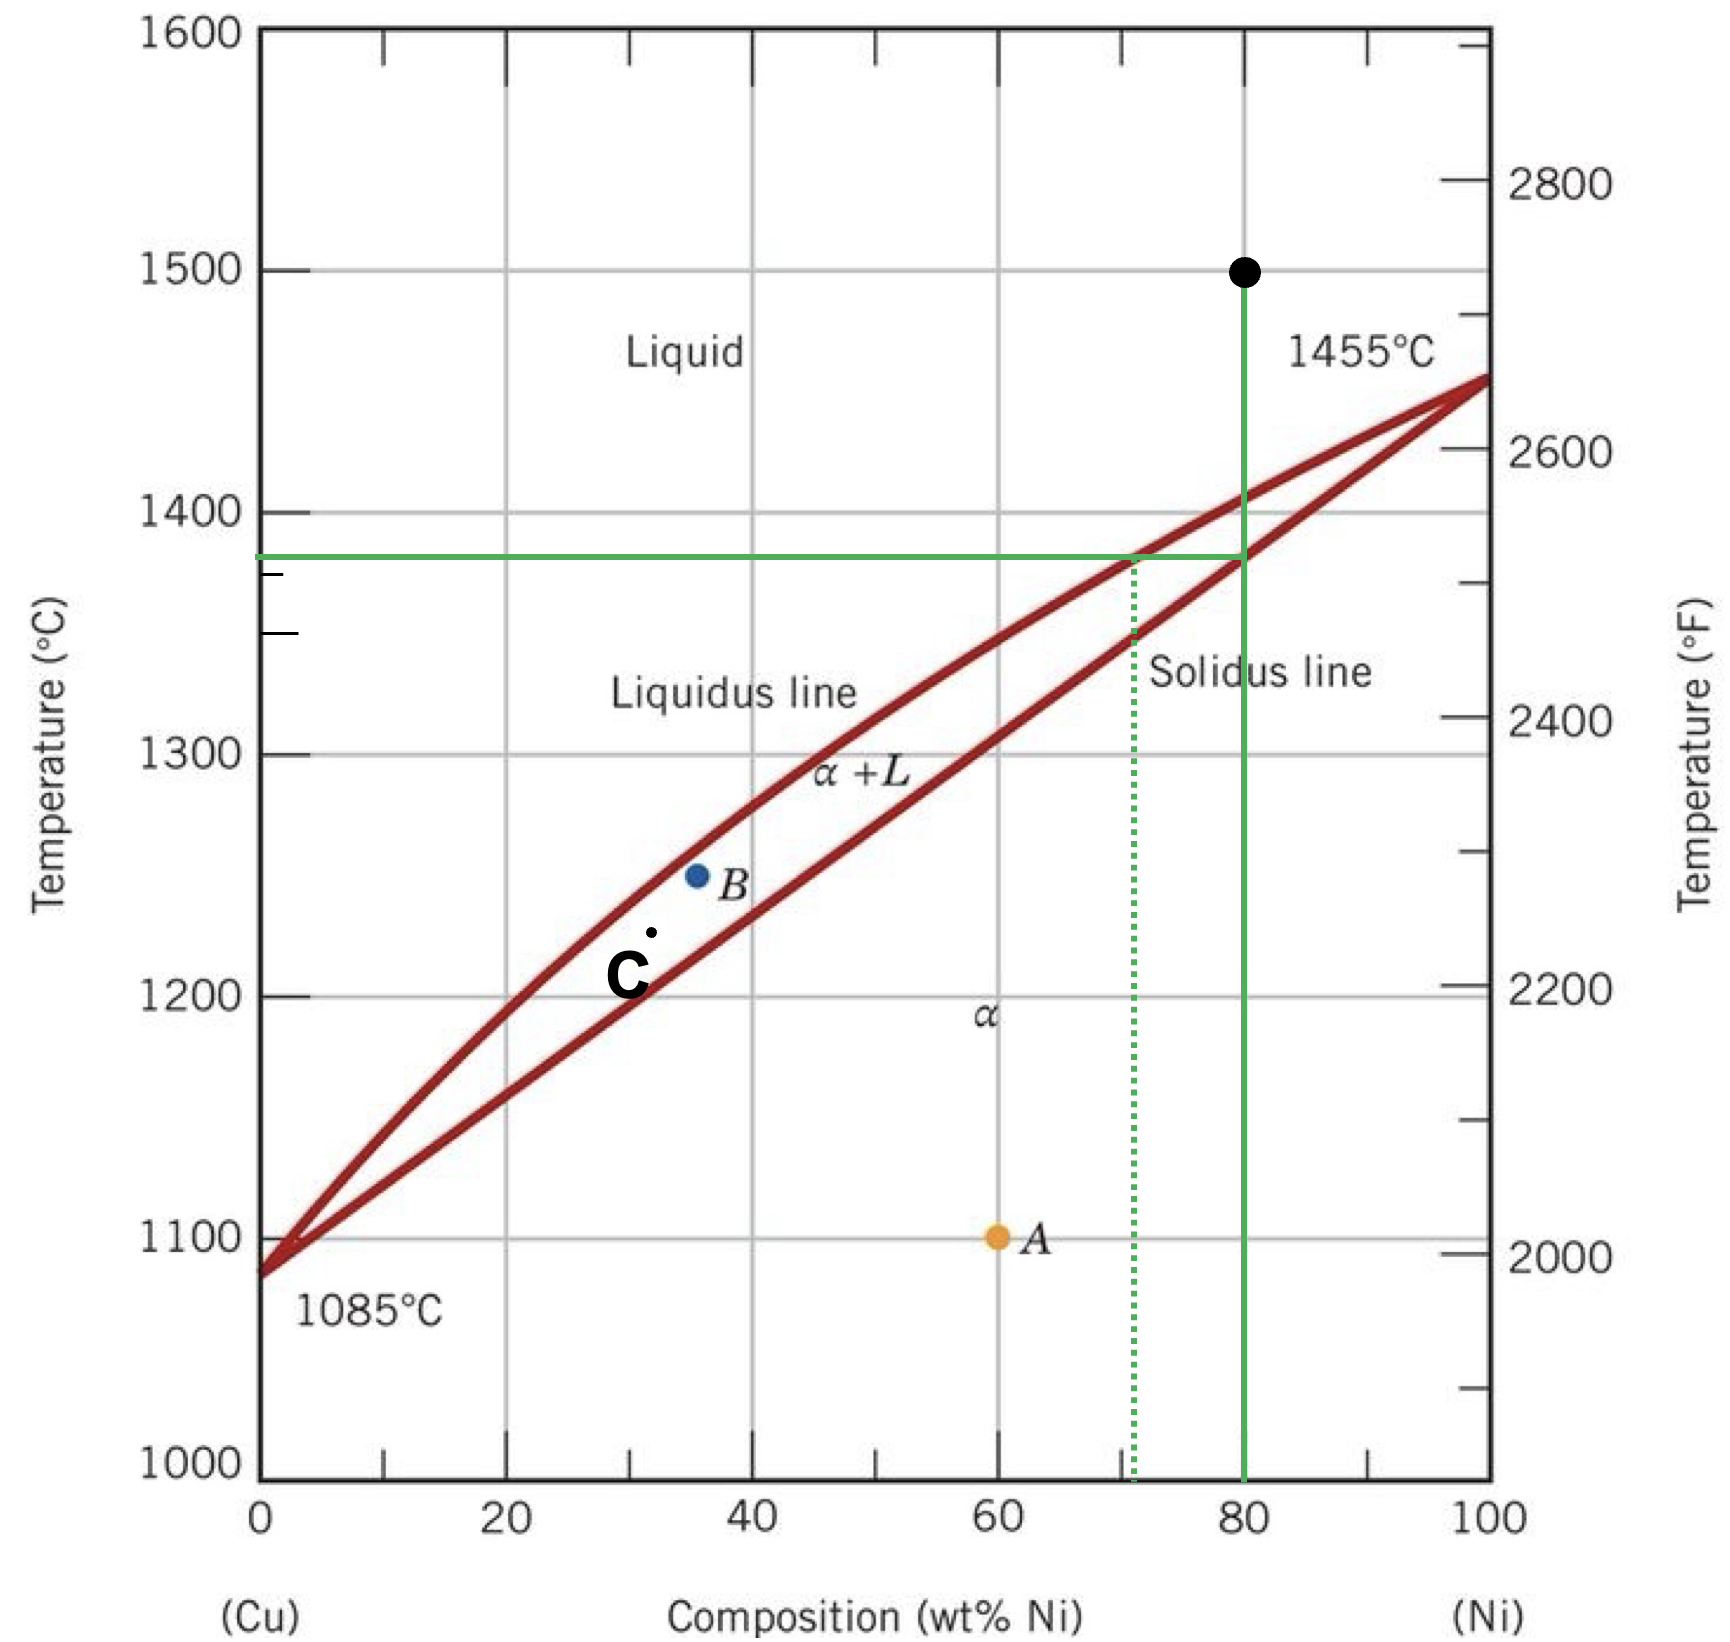
\includegraphics[width=0.7\textwidth]{hw4i2.png}
    \caption{Phase Diagram Showing First Liquid Phase Formation}
\end{figure}

\newpage
\subsection*{Question 1c: Last Solid Phase Prior to Complete Melting (5 points)}
A copper-nickel alloy with a composition of 80 wt\% Ni is slowly heated from room temperature to 1500~$^\circ$C.
\textbf{What is the composition of the last solid phase remaining prior to complete melting, and at what temperature does it completely melt?}

\begin{itemize}
    \item \textbf{Temperature of Complete Melting:} $\sim$1410~$^\circ$C
    \item \textbf{Composition of Last Solid Phase:} $\sim$86 wt\% Ni
\end{itemize}

\noindent\textit{Description of Derivation:} Similar to the previous problem, we draw a vertical line at 80 wt\% Ni until it intersects the liquidus line. We then draw a horizontal line to the temperature axis, determining that the temperature of complete melting is approximately 1410~$^\circ$C. We also use the intersection with the solidus line to draw a vertical line to the composition axis, giving the last solid phase composition as approximately 86 wt\% Ni.

\begin{figure}[h!]
    \centering
    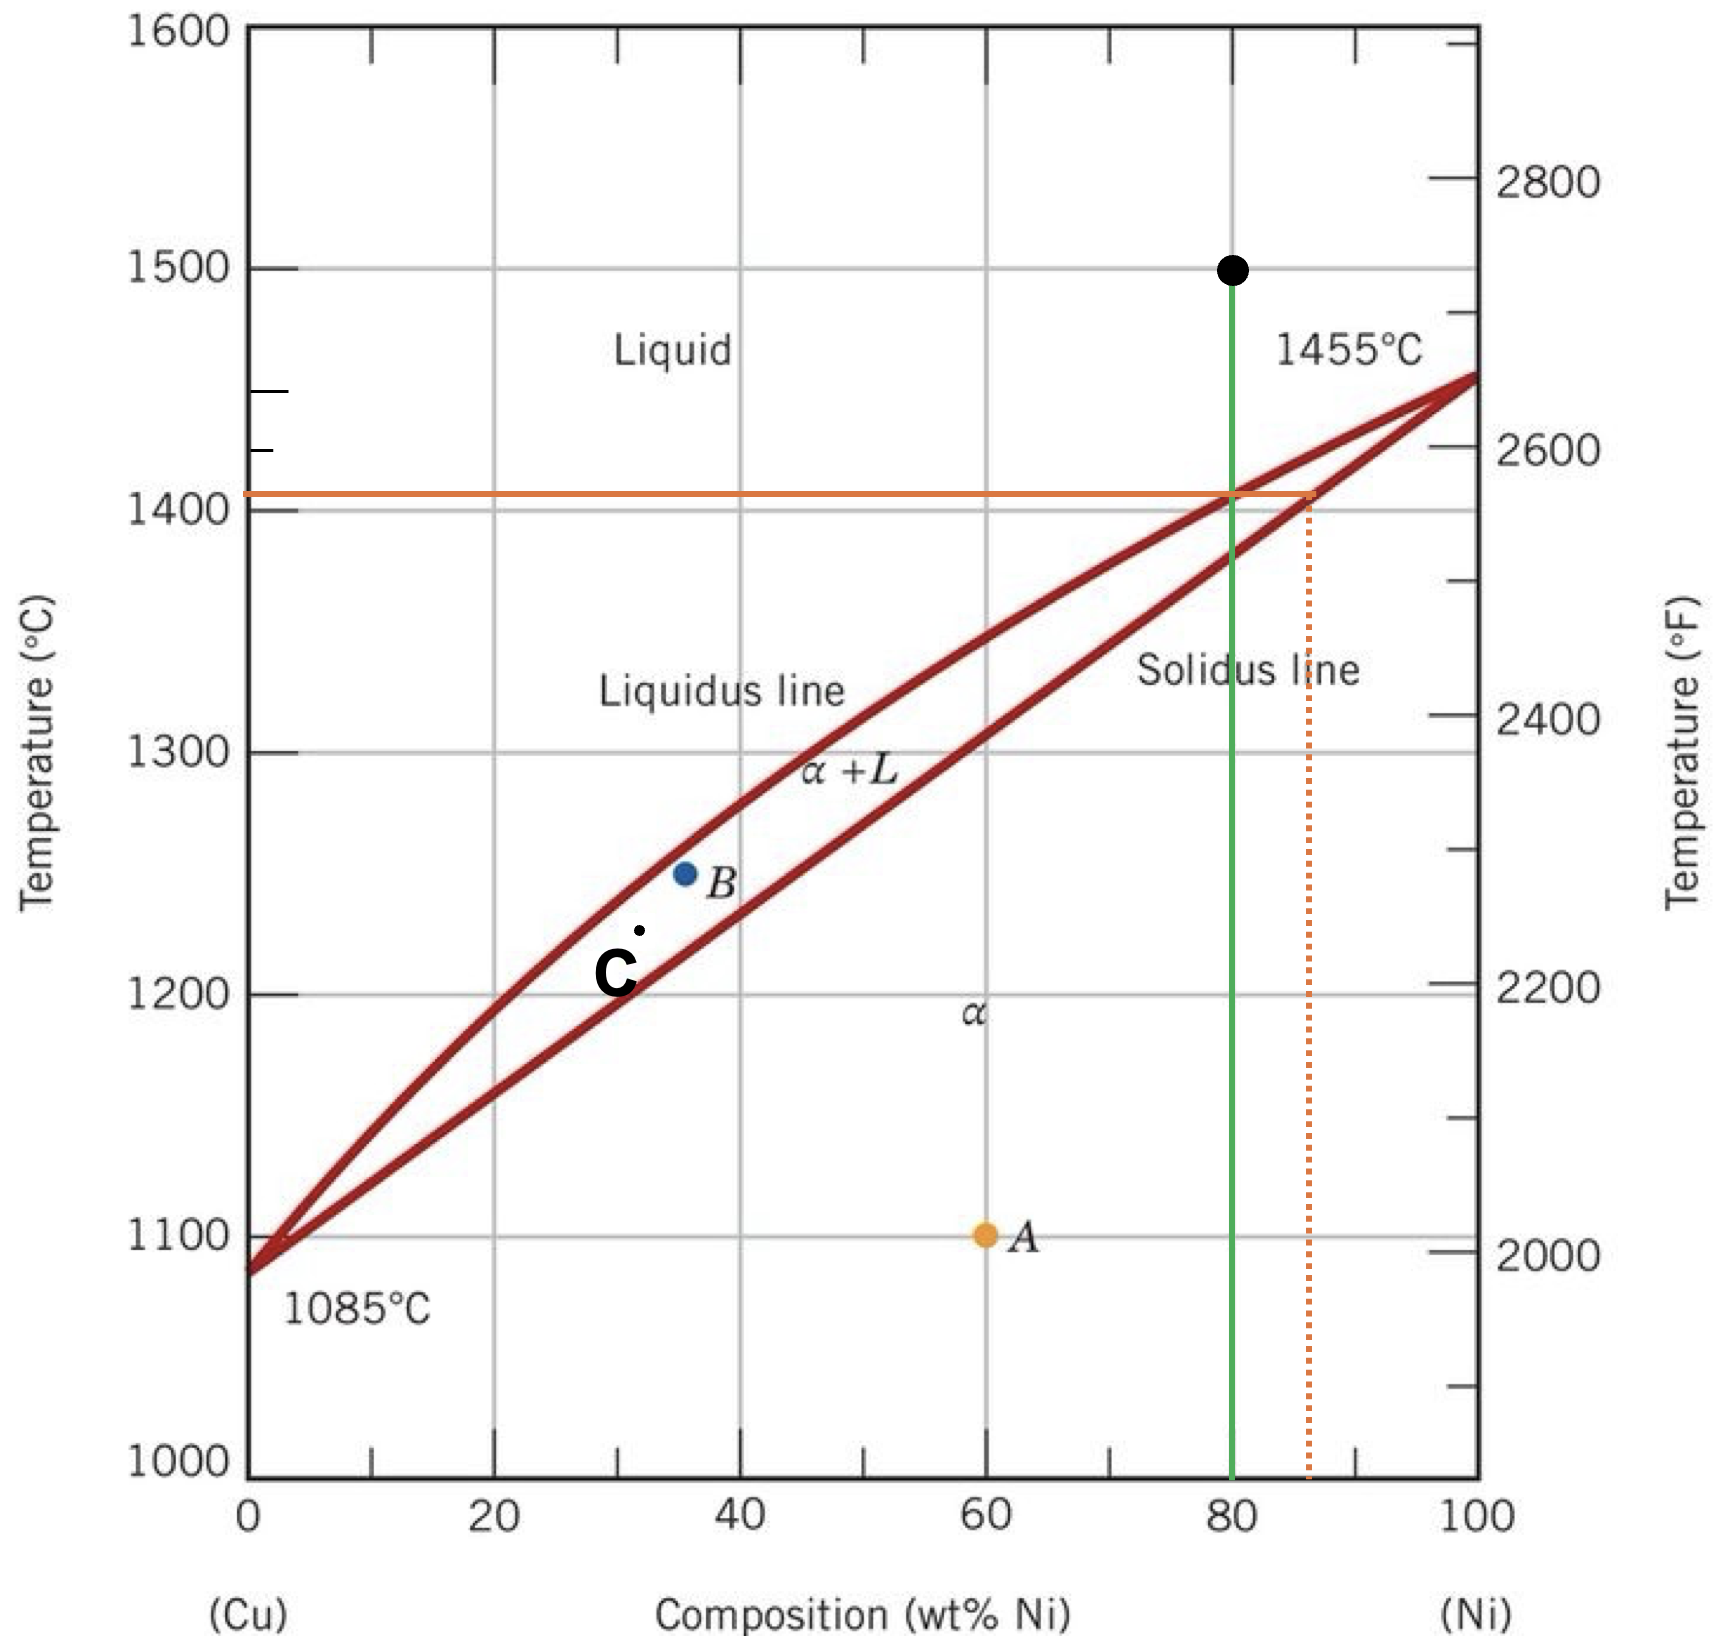
\includegraphics[width=0.7\textwidth]{hw4i3.png}
    \caption{Phase Diagram Showing Last Solid Phase Prior to Complete Melting}
\end{figure}


\newpage \section*{Problem 2}

Consider a 1 kg sample of an Al-Si alloy with 20 wt\% silicon. The sample is slowly cooled from 900°C to room temperature. The Al-Si phase diagram is provided below.

\begin{figure}[h!]
    \centering
    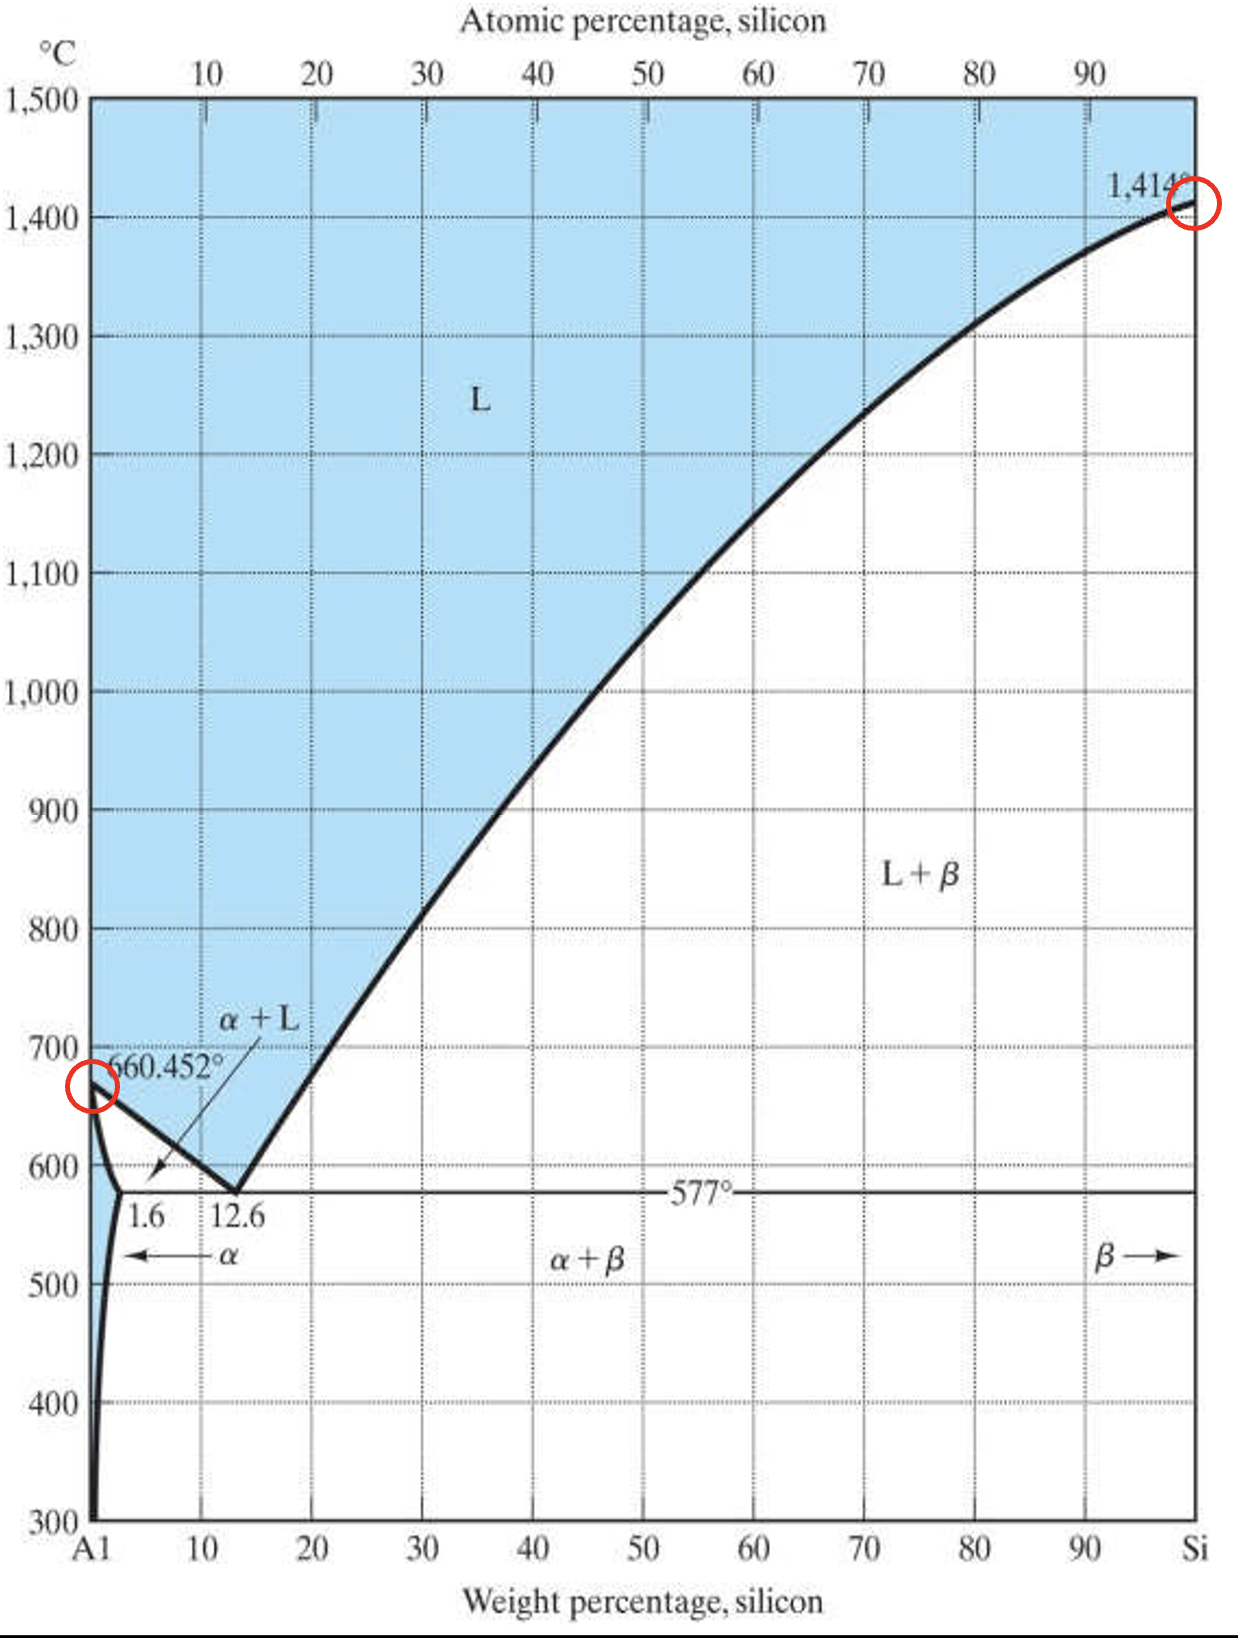
\includegraphics[width=0.6\textwidth]{hw4i4.png}
    \caption{Al-Si Phase Diagram}
    \label{fig:phase-diagram}
\end{figure}

\subsection*{(a) What is the melting point of Al and Si? \hfill (5 points)}

To determine the melting points of aluminum (Al) and silicon (Si), we refer to the phase diagram in Figure~\ref{fig:phase-diagram}.

\begin{itemize}
    \item \textbf{Melting Point of Aluminum (Al):}  
    The melting point of pure aluminum corresponds to the highest temperature on the aluminum-rich side of the phase diagram. From the diagram, aluminum melts at:
    \[
    T_{\text{Al}} = 660.45^\circ\text{C}
    \]
    
    \item \textbf{Melting Point of Silicon (Si):}  
    Similarly, the melting point of pure silicon is found at the highest temperature on the silicon-rich side of the phase diagram. Silicon melts at:
    \[
    T_{\text{Si}} = 1414^\circ\text{C}
    \]
\end{itemize}
\newpage
\subsection*{(b) Upon cooling, at what temperature will the first solid appear, what is the phase of the first solid, and what is the composition of the first solid? \hfill (5 points)}

The temperature at which the first solid appears during cooling is the liquidus temperature. From the phase diagram:

\[
T_{\text{liquidus}} \approx 665^\circ\text{C}
\]

At this temperature, the alloy begins to solidify into two phases:
\begin{itemize}
    \item \textbf{Liquid Phase (L)}
    \item \textbf{Solid Phase ($\beta$)}
\end{itemize}

\textbf{Composition of the First Solid:}  
The $\beta$ phase in the Al-Si system is rich in aluminum. From the phase diagram, the composition of the $\beta$ phase is:
\[
C_{\beta} = 100\% \text{ Al}
\]

\begin{figure}[h!]
    \centering
    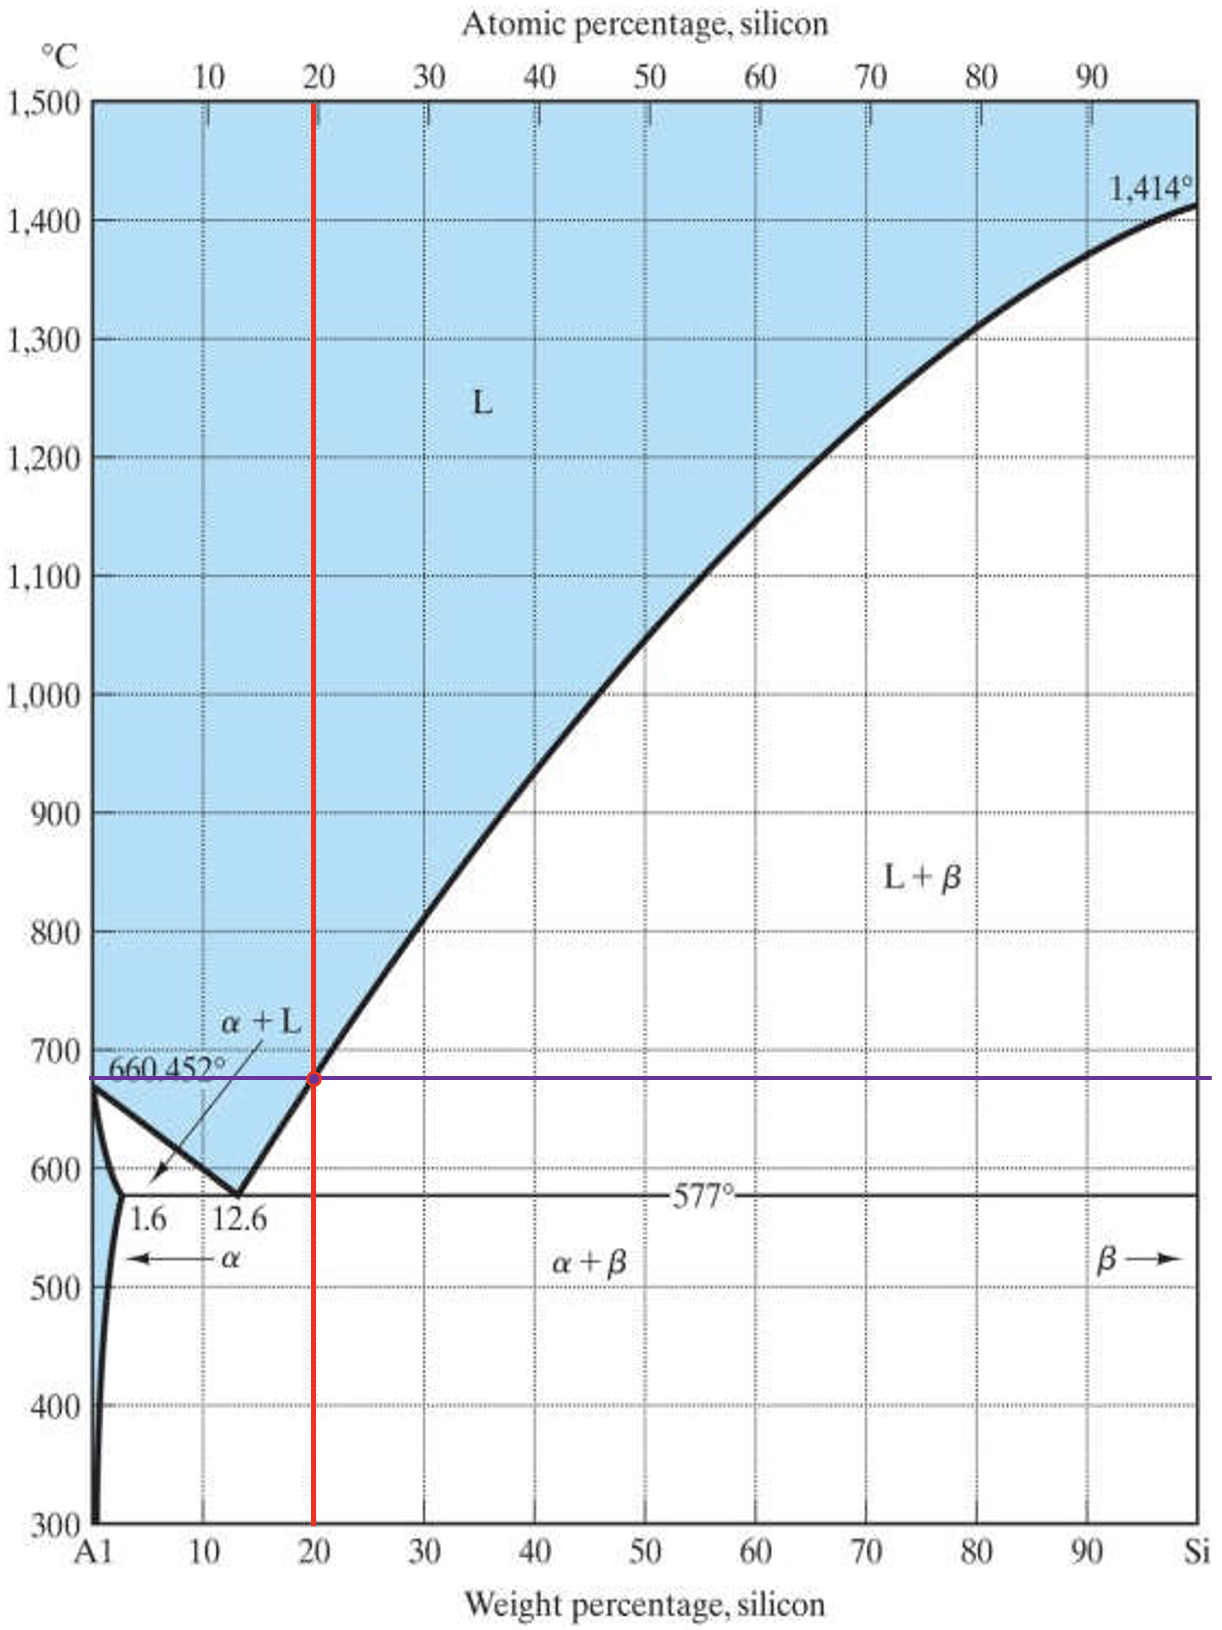
\includegraphics[width=0.6\textwidth]{hw4i5.png}
    \caption{Phase Formation at Liquidus Temperature}
    \label{fig:phase-liquidus}
\end{figure}
\newpage
\subsection*{(c) At 600°C, what phases do you have and what is the mass of each phase? \hfill (10 points)}

At 600°C, the alloy resides in the two-phase region consisting of liquid (L) and the $\beta$ phase. To determine the mass fractions of each phase, we apply the \textbf{Lever Rule}.

\subsubsection*{Given Data}
\begin{itemize}
    \item Total mass of alloy: \( m_{\text{total}} = 1 \text{ kg} \)
    \item Overall composition: \( C_0 = 20\% \text{ Si} \)
    \item Composition of liquid phase at 600°C: \( C_L = 15\% \text{ Si} \)
    \item Composition of $\beta$ phase: \( C_{\beta} = 100\% \text{ Al} \) (which implies \( 0\% \text{ Si} \))
\end{itemize}

\subsubsection*{Applying the Lever Rule}

The Lever Rule equations for the fractions of liquid (\( f_L \)) and solid ($\beta$, \( f_{\beta} \)) phases are:

\[
f_L = \frac{C_{\beta} - C_0}{C_{\beta} - C_L}
\]
\[
f_{\beta} = \frac{C_0 - C_L}{C_{\beta} - C_L}
\]

\subsubsection*{Calculations}

\[
f_L = \frac{100\% - 20\%}{100\% - 15\%} = \frac{80\%}{85\%} \approx 0.941 \text{ (fraction of liquid)}
\]

\[
f_{\beta} = \frac{20\% - 15\%}{100\% - 15\%} = \frac{5\%}{85\%} \approx 0.059 \text{ (fraction of } \beta \text{ phase)}
\]

\subsubsection*{Mass of Each Phase}

\[
\text{Mass of Liquid} = f_L \times m_{\text{total}} = 0.941 \times 1 \text{ kg} = 0.941 \text{ kg}
\]

\[
\text{Mass of } \beta \text{ Phase} = f_{\beta} \times m_{\text{total}} = 0.059 \times 1 \text{ kg} = 0.059 \text{ kg}
\]

\subsubsection*{Summary}

\begin{itemize}
    \item \textbf{Phases Present:} Liquid (L) and $\beta$
    \item \textbf{Mass of Liquid (L):} 0.941 kg
    \item \textbf{Mass of $\beta$ Phase:} 0.059 kg
\end{itemize}

\begin{figure}[h!]
    \centering
    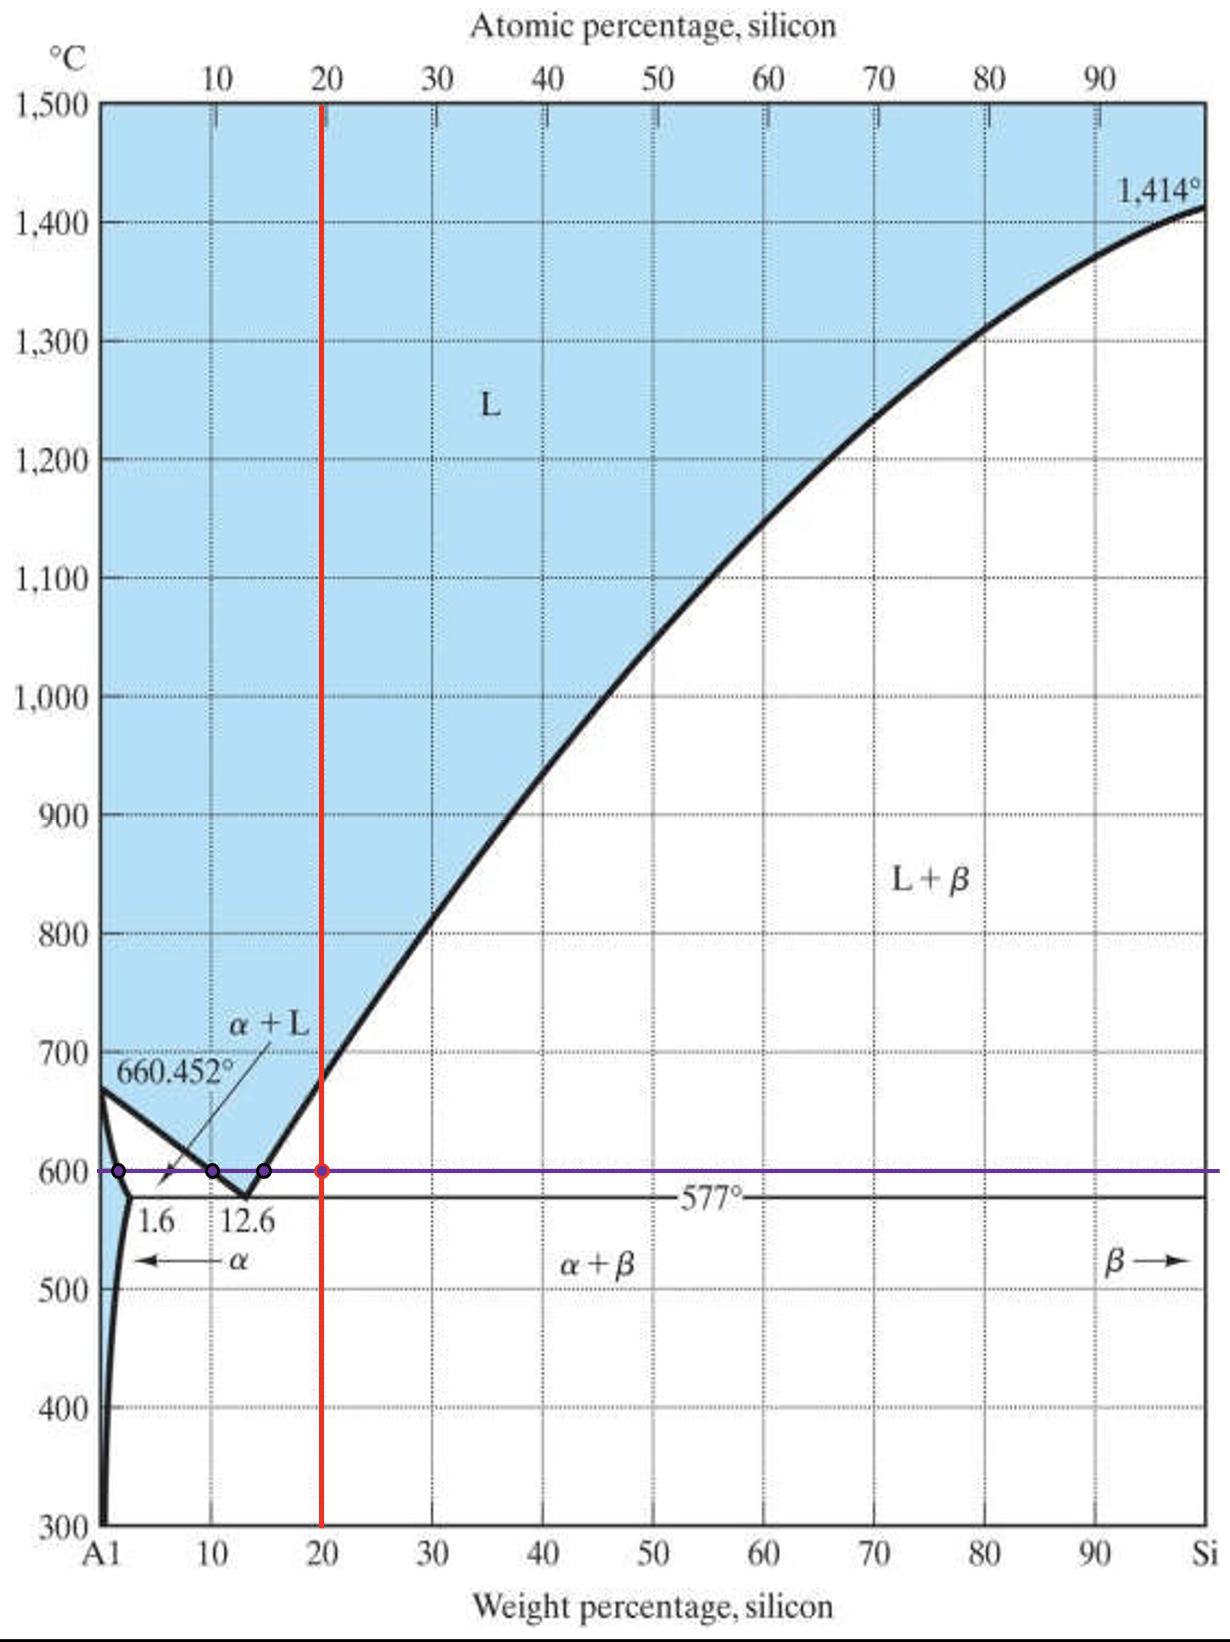
\includegraphics[width=0.6\textwidth]{hw4i6.png}
    \caption{Phase Composition at 600°C}
    \label{fig:phase-600}
\end{figure}
\newpage
\subsection*{(d) At 578°C, what phases do you have and what is the mass of each phase? \hfill (10 points)}

At 578°C, the alloy remains in the two-phase region of liquid (L) and the $\beta$ phase. We use the Lever Rule to determine the mass fractions.

\subsubsection*{Given Data}
\begin{itemize}
    \item Total mass of alloy: \( m_{\text{total}} = 1 \text{ kg} \)
    \item Overall composition: \( C_0 = 20\% \text{ Si} \)
    \item Composition of liquid phase at 578°C: \( C_L = 12.6\% \text{ Si} \)
    \item Composition of $\beta$ phase: \( C_{\beta} = 100\% \text{ Al} \) (which implies \( 0\% \text{ Si} \))
\end{itemize}

\subsubsection*{Applying the Lever Rule}

\[
f_L = \frac{C_{\beta} - C_0}{C_{\beta} - C_L} = \frac{100\% - 20\%}{100\% - 12.6\%} = \frac{80\%}{87.4\%} \approx 0.915 \text{ (fraction of liquid)}
\]

\[
f_{\beta} = \frac{C_0 - C_L}{C_{\beta} - C_L} = \frac{20\% - 12.6\%}{100\% - 12.6\%} = \frac{7.4\%}{87.4\%} \approx 0.085 \text{ (fraction of } \beta \text{ phase)}
\]

\subsubsection*{Mass of Each Phase}

\[
\text{Mass of Liquid} = f_L \times m_{\text{total}} = 0.915 \times 1 \text{ kg} = 0.915 \text{ kg}
\]

\[
\text{Mass of } \beta \text{ Phase} = f_{\beta} \times m_{\text{total}} = 0.085 \times 1 \text{ kg} = 0.085 \text{ kg}
\]

\subsubsection*{Summary}

\begin{itemize}
    \item \textbf{Phases Present:} Liquid (L) and $\beta$
    \item \textbf{Mass of Liquid (L):} 0.915 kg
    \item \textbf{Mass of $\beta$ Phase:} 0.085 kg
\end{itemize}

\begin{figure}[h!]
    \centering
    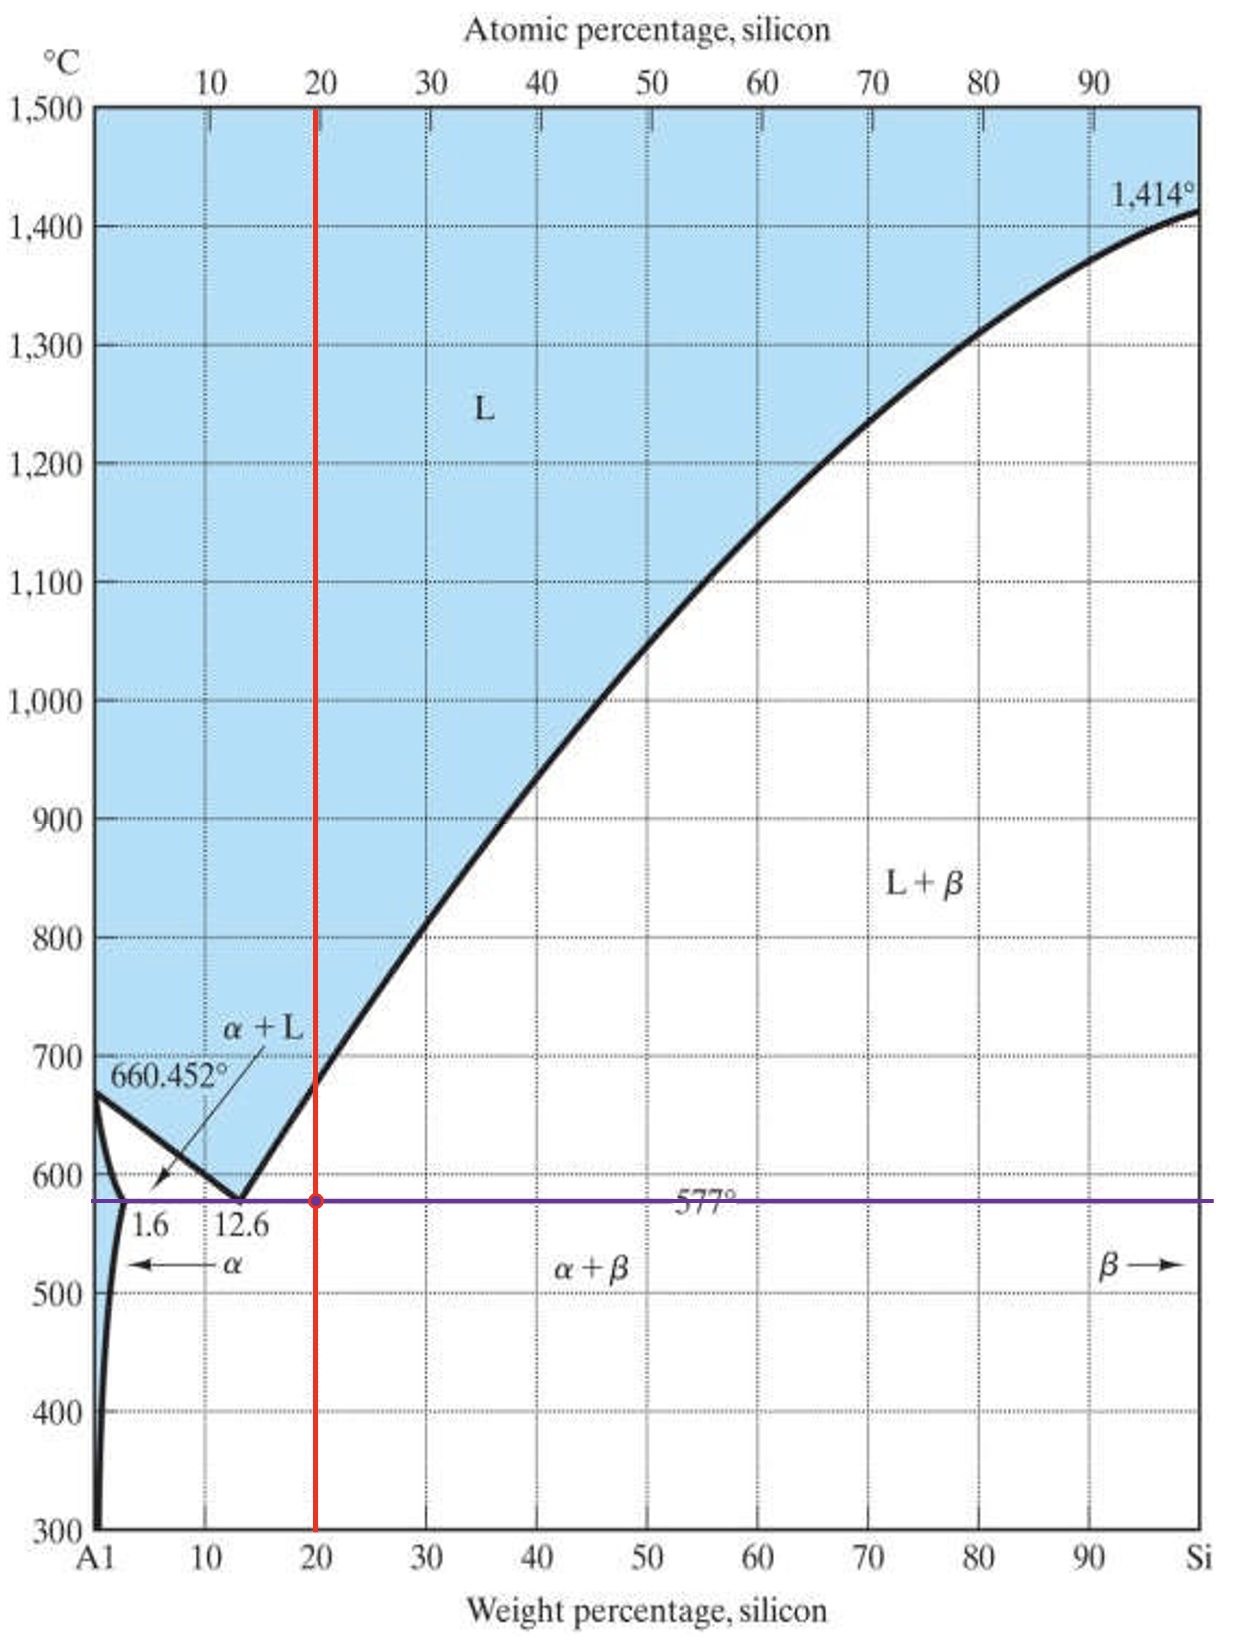
\includegraphics[width=0.6\textwidth]{hw4i7.png}
    \caption{Phase Composition at 578°C}
    \label{fig:phase-578}
\end{figure}
\newpage

\section*{Problem 3}
(Total 15 points)

The Al-Si phase diagram is provided below. Consider a 1 kg sample of an Al-Si alloy with 80 wt\% silicon. The sample is slowly heated from room temperature to 1400°C. Upon cooling, answer the following questions.

\begin{figure}[h]
    \centering
    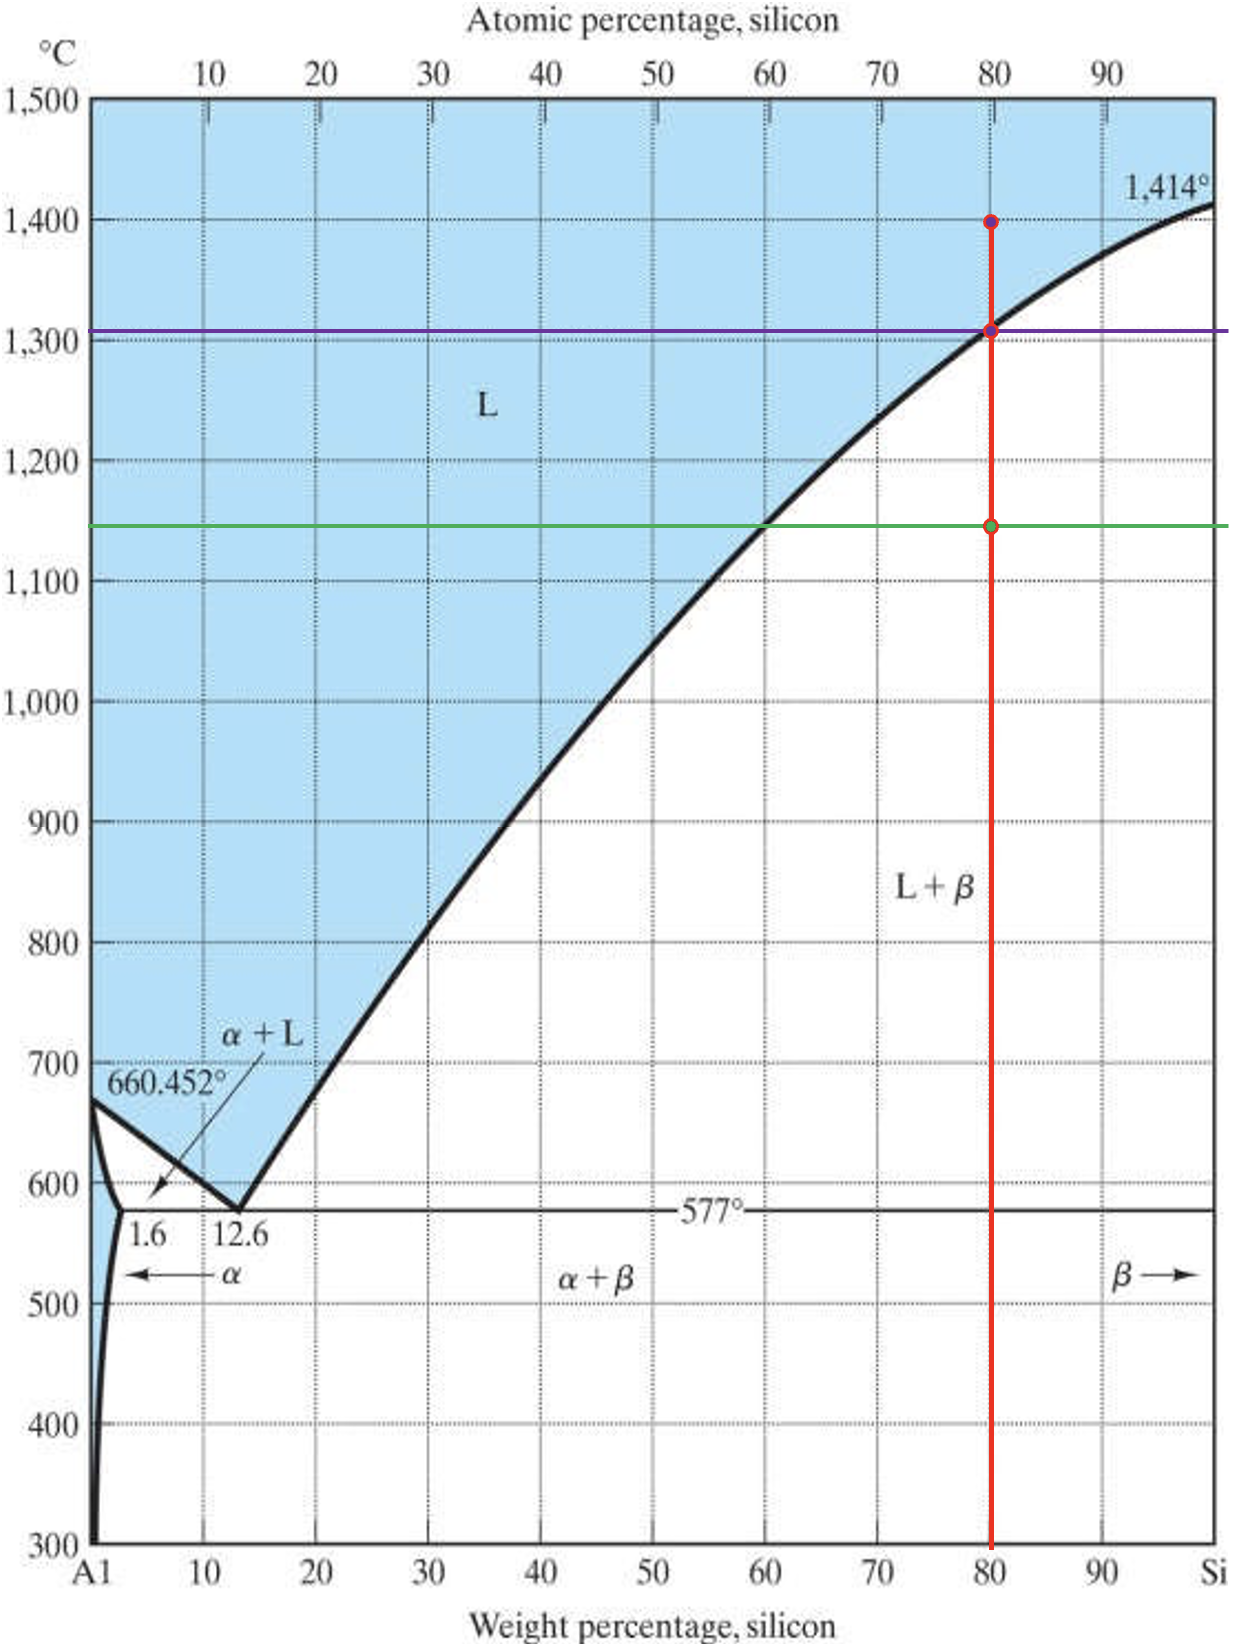
\includegraphics[width=0.6\textwidth]{hw4i8.png}
    \caption{Al-Si Phase Diagram}
    \label{fig:phase-diagram-3}
\end{figure}

\subsection*{(i) At what temperature will the liquid start to solidify and what is the composition of the first solid formed? }
\subsubsection*{Solution}

\textbf{Determining the Liquidus Temperature:}

To find the temperature at which the liquid begins to solidify (the liquidus temperature), we refer to the Al-Si phase diagram in Figure~\ref{fig:phase-diagram-3}. For an alloy with 80 wt\% silicon, we locate this composition on the horizontal axis and identify the corresponding liquidus temperature.

\[
T_{\text{liquidus}} = 1310^\circ\text{C}
\]

\textbf{Phase of the First Solid Formed:}

At the liquidus temperature, the first solid that begins to form from the liquid is the $\beta$-phase. According to the phase diagram, the $\beta$-phase in the Al-Si system is pure silicon.

\[
\text{Composition of } \beta\text{-phase} = 100\% \text{ Si}
\]

\subsection*{(ii) At what temperature will you have an equal amount of solid and liquid phase? And what is the composition of the liquid phase at this temperature?}

\subsubsection*{Solution}

\textbf{Determining the Temperature for Equal Amounts of Solid and Liquid:}

To find the temperature at which the mass of the solid phase equals the mass of the liquid phase, we identify the eutectic temperature or the temperature where the lever rule indicates a 1:1 ratio of phases. From the phase diagram, for an 80 wt\% Si alloy, this temperature is:

\[
T = 1140^\circ\text{C}
\]


\subsubsection*{From Diagram}
\begin{itemize}
    \item Overall composition: \( C_0 = 80\% \text{ Si} \)
    \item Composition of liquid phase at $1140^\circ\text{C}$: \( C_L = 60\% \text{ Si} \)
    \item Composition of $\beta$-phase: \( C_{\beta} = 100\% \text{ Si} \)
\end{itemize}
\newpage
\section*{Problem 4}

Consider 1 kg of a Pb-Sn alloy with 50 wt\% Sn. The alloy is heated to 400°C.

\begin{figure}[h]
    \centering
    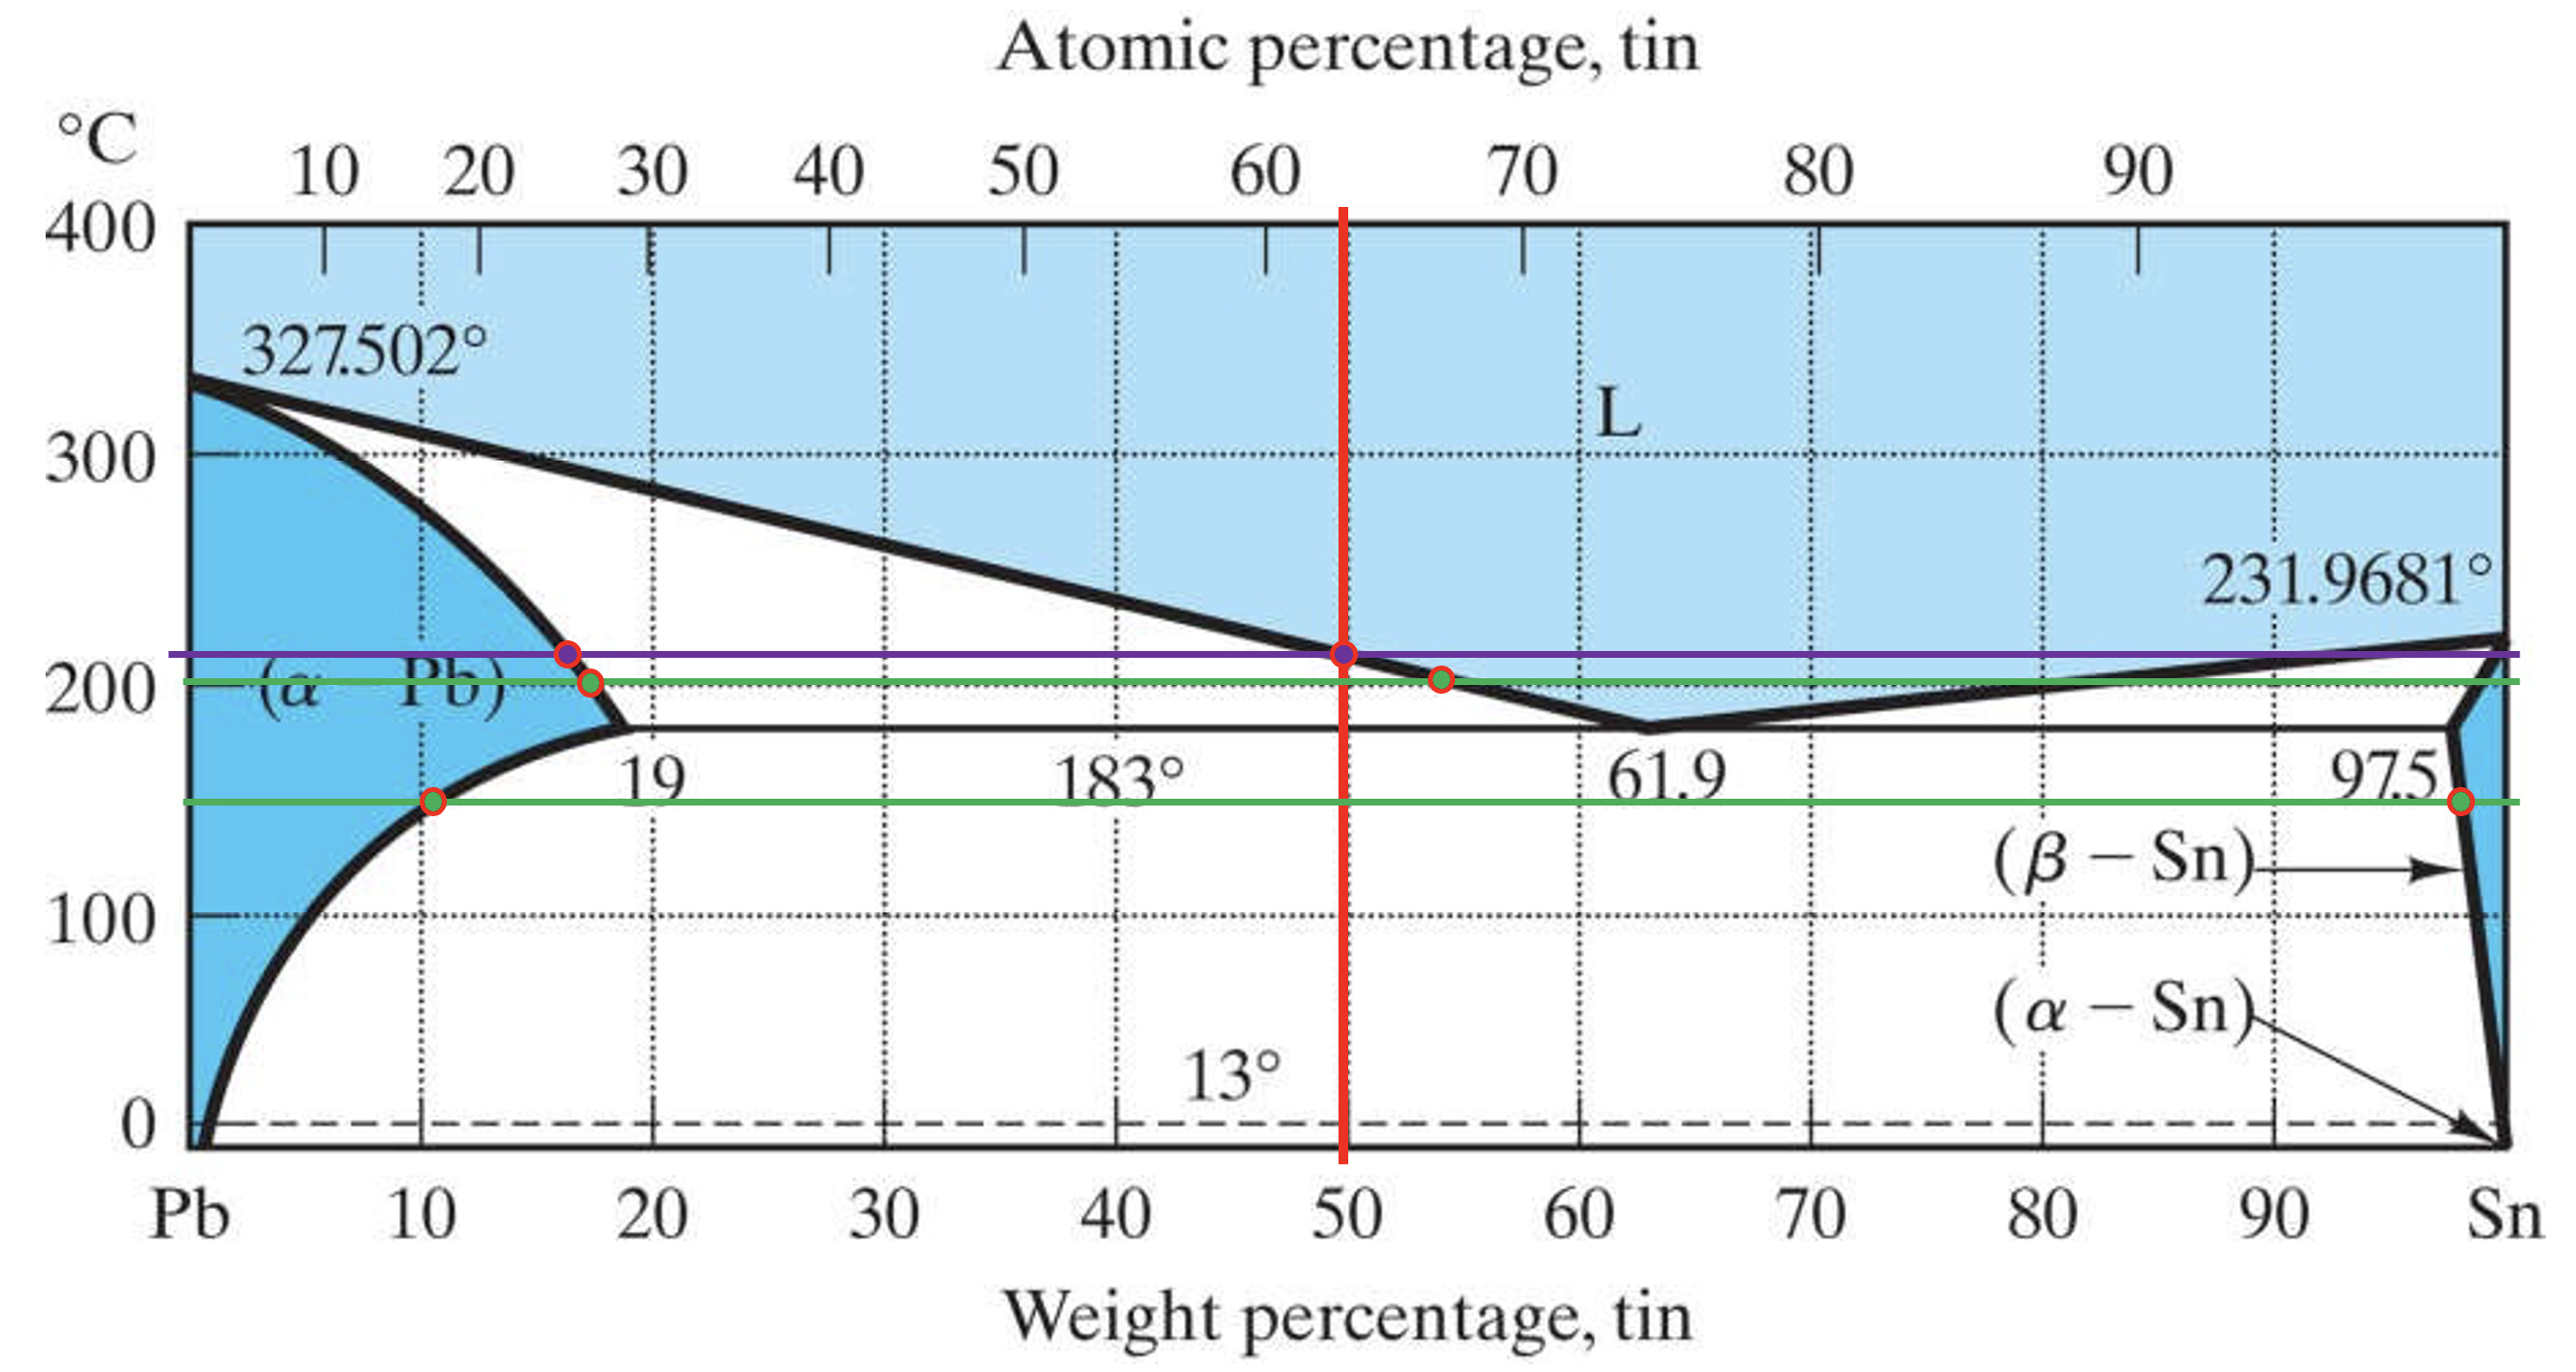
\includegraphics[width=0.8\textwidth]{hw4i9.png}
    \caption{Pb-Sn Phase Diagram}
    \label{fig:hw4i9}
\end{figure}

\begin{enumerate}

\item \textbf{Upon cooling, at what temperature will the first solid appear, what is the phase of the first solid, and what is its composition?} \hfill \textbf{(5 points)}

\textbf{Answer:}

\begin{itemize}
    \item \textbf{Temperature of first solid appearance:} 210°C
    \item \textbf{Phase of the first solid:} $\alpha$-Pb
    \item \textbf{Composition of the first solid:} 16 wt\% Sn
\end{itemize}

\item \textbf{At 200°C, you have a mixture of solid and liquid phases. Is the amount of the solid phase more than, equal to, or less than the amount of the liquid phase? Justify your answer.} \hfill \textbf{(10 points)}

\textbf{Answer:}

Since the overall composition of 50 wt\% Sn is closer to the liquidus composition than to the $\alpha$-Pb phase composition, the alloy contains a larger proportion of the liquid phase compared to the solid phase. Therefore, the amount of the solid phase is \textbf{less than} the amount of the liquid phase.

\item \textbf{At 150°C, the alloy consists of two solid phases, $\alpha$-Pb and $\beta$-Sn. Is the amount of the $\alpha$-Pb solid phase greater than, equal to, or less than the amount of the $\beta$-Sn solid phase?} \hfill \textbf{(5 points)}

\textbf{Answer:}

The $\beta$-Sn phase composition is farther from the overall alloy composition than the $\alpha$-Pb phase. This implies that more of the $\alpha$-Pb phase is required to balance the overall composition. Therefore, the amount of the $\alpha$-Pb solid phase is \textbf{greater than} the amount of the $\beta$-Sn solid phase.

\end{enumerate}


\newpage

\subsection*{Problem 5: Heating and Cooling Low Carbon Steel}
Heating 1 pound of a common low carbon steel with 0.50 wt\% C content to 1000\(^\circ\)C and then slowly cooling it down to room temperature. The iron phase diagram is shown below.

\subsection*{(a) Eutectic Temperature, Composition, and Reaction (5 points)}
\begin{itemize}
    \item \textbf{Eutectic Temperature:} 1148 \(^\circ\)C
    \item \textbf{Eutectic Composition:} 4.30 wt\% C - 95.7 wt\% Fe
    \item \textbf{Eutectic Reaction:}
    \begin{equation*}
        L \overset{\text{cool}}{\underset{\text{heat}}{\longleftrightarrow}} \gamma + \text{Fe}_3\text{C}
    \end{equation*}
\end{itemize}

\subsection*{(b) Eutectoid Temperature, Composition, and Reaction (5 points)}
\begin{itemize}
    \item \textbf{Eutectoid Temperature:} 727 \(^\circ\)C
    \item \textbf{Eutectoid Composition:} 0.77 wt\% C - 99.23 wt\% Fe
    \item \textbf{Eutectoid Reaction:}
    \begin{equation*}
        \gamma \overset{\text{cool}}{\underset{\text{heat}}{\longleftrightarrow}} \alpha + \text{Fe}_3\text{C}
    \end{equation*}
\end{itemize}

\subsection*{(c) At 728°C: Phases and Mass of Each Phase (5 points)}
\begin{itemize}
    \item \textbf{Phases Present:} \(\gamma\) (austenite) and \(\alpha\) (ferrite).
    \item \textbf{Compositions of the Phases:}
    \begin{itemize}
        \item Composition of \(\gamma\): 0.77 wt\% C.
        \item Composition of \(\alpha\): 0.02 wt\% C.
    \end{itemize}
    \item \textbf{Lever Rule to Find Mass Fractions:}
    \begin{align*}
        f_\gamma &= \frac{C_0 - C_\alpha}{C_\gamma - C_\alpha} = \frac{0.50 - 0.02}{0.77 - 0.02} = \frac{0.48}{0.75} \approx 0.64 \\
        f_\alpha &= \frac{C_\gamma - C_0}{C_\gamma - C_\alpha} = \frac{0.77 - 0.50}{0.77 - 0.02} = \frac{0.27}{0.75} \approx 0.36
    \end{align*}
    \item \textbf{Mass of Each Phase:}
    \begin{align*}
        m_\gamma &= f_\gamma \times 1 \, \text{lb} = 0.64 \, \text{lb}, \\
        m_\alpha &= f_\alpha \times 1 \, \text{lb} = 0.36 \, \text{lb}.
    \end{align*}
\end{itemize}

\subsection*{(d) At Room Temperature: Phases and Mass of Each Phase (5 points)}
\begin{itemize}
    \item \textbf{Phases Present:} \(\alpha\) (ferrite) and \(\text{Fe}_3\text{C}\) (cementite).
    \item \textbf{Compositions of the Phases:}
    \begin{itemize}
        \item Composition of \(\alpha\): 0.02 wt\% C.
        \item Composition of \(\text{Fe}_3\text{C}\): 6.69 wt\% C.
    \end{itemize}
    \item \textbf{Lever Rule to Find Mass Fractions:}
    \begin{align*}
        f_\alpha &= \frac{C_\text{Fe3C} - C_0}{C_\text{Fe3C} - C_\alpha} = \frac{6.69 - 0.50}{6.69 - 0.02} = \frac{6.19}{6.67} \approx 0.93 \\
        f_\text{Fe3C} &= \frac{C_0 - C_\alpha}{C_\text{Fe3C} - C_\alpha} = \frac{0.50 - 0.02}{6.69 - 0.02} = \frac{0.48}{6.67} \approx 0.07
    \end{align*}
    \item \textbf{Mass of Each Phase:}
    \begin{align*}
        m_\alpha &= f_\alpha \times 1 \, \text{lb} = 0.93 \, \text{lb}, \\
        m_\text{Fe3C} &= f_\text{Fe3C} \times 1 \, \text{lb} = 0.07 \, \text{lb}.
    \end{align*}
\end{itemize}
\end{document}
